\documentclass[10pt]{article}
% Standard packages
% \usepackage[paperwidth=14.in, paperheight=18in, top= 0.5in, bottom=0.5in, right=0.5in, left=0.5in]{geometry}

\usepackage{pgfkeys}
\usepackage{tabu}
\usepackage{multirow}
\usepackage{caption}
\usepackage{listings}
\usepackage{xcolor}
\usepackage{float}
\usepackage{verbatim}

\definecolor{codegreen}{rgb}{0,0.6,0}
\definecolor{codegray}{rgb}{0.5,0.5,0.5}
\definecolor{codepurple}{rgb}{0.58,0,0.82}
\definecolor{backcolour}{rgb}{0.95,0.95,0.92}
 
\lstdefinestyle{mystyle}{
    backgroundcolor=\color{backcolour},   
    commentstyle=\color{codegreen},
    keywordstyle=\color{magenta},
    numberstyle=\tiny\color{codegray},
    stringstyle=\color{codepurple},
    basicstyle=\ttfamily\footnotesize,
    breakatwhitespace=false,         
    breaklines=true,                 
    captionpos=b,                    
    keepspaces=true,                 
    numbers=left,                    
    numbersep=5pt,                  
    showspaces=false,                
    showstringspaces=false,
    showtabs=false,                  
    tabsize=2
}
 
\lstset{style=mystyle}
% Required packages for tikz-uml
\usepackage{graphicx}
\usepackage{tikz}
\usetikzlibrary{positioning}
\usepackage{ifthen}
\usepackage{xstring}
\usepackage{calc}
\usepackage{pgfplots}
\usepackage{hyperref}

\newcommand{\dunder}{\rule{0.1in}{0.1pt}}
\newcommand{\Newpage}{\end{preview}\begin{preview}}
\newcommand{\setvalue}[1]{\pgfkeys{/variables/#1}}
\newcommand{\getvalue}[1]{\pgfkeysvalueof{/variables/#1}}
\newcommand{\declare}[1]{%
 \pgfkeys{
  /variables/#1.is family,
  /variables/#1.unknown/.style = {\pgfkeyscurrentpath/\pgfkeyscurrentname/.initial = ##1}
 }%
}
\usepackage[margin=1in]{geometry}
\setlength{\parskip}{\baselineskip}%
\setlength{\parindent}{0pt}%

\title{APC524 Final Project Report}
% Name
\author{Bruun, E. \and Flores, J. \and Kumar, V.}


\begin{document}
\maketitle

\section{Introduction}
\label{sec:intro}
	\subsection{Scientific Background}
		Rapidly-exploring random trees (RRTs) are a class of algorithms used in autonomous robotic motion planning to efficiently calculate a path through a large unsearched domain. This domain can either represent a physical space (i.e. 2D or 3D Euclidean space), or a higher-dimensional robotic state space. The algorithm generates trajectories through the domain, and can easily handle multiple obstacles, goals, or other differential constraints that are applicable to a robotic motion planning problem.
		
		The RRT works by growing a search tree incrementally from random samples drawn from the domain, and is therefore biased to grow into unsearched areas. As a new sample is drawn, the algorithm attempts to connect it to the nearest point in the existing solution-path tree. If the connection is possible (i.e. does not collide with an obstacle, or is otherwise infeasible from a kinematic perspective) then a new graph edge is made and the next iteration begins.
		
		The Basic RRT algorithm was first proposed by Lavalle and Kuffner in 1998. While its development was a paradigm shift in the field of robotic motion planning (RRTs were significantly more efficient than the existing path planning methods), the main drawback of the Basic RRT is that it almost surely converges to a non-optimal value. Since the proposal of the Basic RRT, developing new algorithms modifying its underlying principles has been an active area of research. The most significant leap forward was the development of the RRT* (RRT Star) algorithm by Frazzoli in 2010, which is a variant of the Basic RRT that guarantees convergence to the optimal solution.

	\subsection{Motivation}
		The goal of this project is to develop a modular and scalable program that implements a variety of path-planning algorithms to search through a physical domain space populated with obstacles. The ultimate motivation for this work is to assess the relative efficiency and performance of a large set of different algorithms acting in various domains. Therefore, the program is developed in such a way that both the definition of the domain space, and the solution procedure is extensible in the future. 


	\subsection{Program Limitations}
		Currently only the Basic RRT and the RRT* algorithms are implemented. But examining the difference between these two algorithms is an adequate starting point for showing the difference between a random search method and one that approaches optimality.
		
		Currently only a 2D physical domain space has been implemented. The domain can only be a regular shape (circle or rectangle)
		
		Currently only bitmap (.pbm) shapes can be used to define any freeform (i.e. not regular shapes) obstacles or goals to be placed inside the domain.

\newpage
\section{Development Process}
\label{sec:dev_process}
As highlighted in section~\ref{sec:intro} and design document, the key components of this software are geometrical set up (domain and obstacles), algorithm for path finding, solution method and results visualization. The goal of this project was to develop a modular and extensible path find software and the development process was decided based on this goal. The aforementioned tasks were divided amongst the group members, who were responsible for a given set of classes. Git was used for maintaining the collaborative work amongst the members. As tasks were fairly independent, it was important to have unit tests as well as integration tests to make sure that the software was working in a cohesive manner. Evolution of the software required automatic testing applications to make sure new additions did not break it. Along the way, various issues were faced and lesson learned. The whole processes is detailed in the following subsections.
\subsection{Github Repo Setup}
Given the flexibility offered by Git, it is unsurprising that various recipes for collaborative work have emerged over the years. A few common workflow models are:
\begin{enumerate}
	\item \href{https://www.atlassian.com/git/tutorials/comparing-workflows#centralized-workflow}{Centralized Workflow}: Only one branch {\ttfamily master} is used and all the team members commit changes to this branch. This option is however prone to merge conflicts.
	\item \href{https://www.atlassian.com/git/tutorials/comparing-workflows/feature-branch-workflow}{Feature Branch Workflow}: The core idea behind this approach is that any new feature development takes place on a dedicated branch which means that the {\ttfamily master} branch is never broken. Further this allows for pull requests which help to discuss the code before they are pushed to {\ttfamily master}.
	\item \href{https://www.atlassian.com/git/tutorials/comparing-workflows/gitflow-workflow}{Gitflow Workflow}: Popularized by Vincent Drienssen at \href{https://nvie.com/posts/a-successful-git-branching-model/}{nvie} this is used in larger projects which are focused on software release cycles. A {\ttfamily develop} branch is created from {\ttfamily master} which is used to create {\ttfamily feature} and {\ttfamily release} branches. Branch {\ttfamily feature} is merged to {\ttfamily develop}, while {\ttfamily release} is also merged with {\ttfamily master}. It further allows for a {\ttfamily hotfixe} branch to resolve issues with master.
	\item \href{https://www.atlassian.com/git/tutorials/comparing-workflows/forking-workflow}{Forking Workflow}: Commonly used in open source projects (e.g. \href{https://github.com/dealii/dealii}{DEAL.II}), this model gives each developer their own server-side repository. Only the maintainers of the software have write access to the official code, while giving contributors an option to create pull requests to add features to the open source project.
\end{enumerate}
Since there are only three developers involved in this project who communicated frequently in person, a mix of "Gitflow" and "Feature Branch" workflows was adopted. The rationale being that each one of us is responsible for a given feature and only merges with {\ttfamily development} branch if all the tests pass. One of the members was responsible for integration tests and to merge the {\ttfamily development} with {\ttfamily master}. This was a nice middle ground between the rigorous checks of option 3 and 4, and a complete mayhem that could result from working on master branch directly. The work flow of the software development can be best visualized as shown in the Figure~\ref{fig:git_structure}.
\begin{figure}[H]
	\centering
	\includegraphics[width=0.9\textwidth]{./figures/git_work_flow.pdf}
	\caption{\label{fig:git_structure} Graph demonstrating the git work-flow between the developers}
\end{figure}
\subsection{Writing Tests}
For the purpose of this project, unit tests were written to evaluate the various classes for expected behavior and determining edge cases. The project was not entirely test-driven, i.e. the tests were not written before the code, but rather tests were written along with the creation of new classes as well as whenever the functionality of a class changed. To make sure that the functionality of the software was never compromised, it was mandated that all the tests must pass before the code could be pushed to the {\ttfamily development} branch. The tests had another benefit of informing the team members about the input parameters required and the methods and attributes to expect. This became highly important as the classes evolved and deviated from our initial design proposal. Two different approaches to writing tests were taken by the team members. This was because we did not decide on a preferred method and by the time we caught on there was an inertia to change it. The two approaches were:
\begin{enumerate}
	\item \href{https://docs.python.org/3.6/library/unittest.html#module-unittest}{unittest}: The unittest module of python was used to test the algorithms and the solver classes. These classes were complex and depended on a number of other classes
	\item \href{https://docs.pytest.org/en/latest/}{pytest}: Pytest was used for the tests of input modules, such as domain, obstacles and shapes. As these objects were fairly simple and had similar functionalities, it was best to write simple tests to expose edge cases.
\end{enumerate}
The key takeaways were:
\begin{enumerate}
\item The tests helped us communicate our ideas for individual classes clearly. The tests explicitly detailed what were the expected functionalities of each class. If an improvement was required, it was easy to communicate to the relevant person.
\item Initially, it was easy to skip the testing and go ahead with adding functionalities to the code as it was our first real attempt at test driven software development. Over time however, the process became more streamlined.
\end{enumerate}
\subsection{Travis}
To deploy continuous integration \href{https://travis-ci.com}{Travis} was the platform of choice. The tests were run using python versions 3.6 to 3.8-dev. This was added much later in the project stage as we were not able to add it to the private repository under the Princeton University organization. Through email communications, it appeared that any repository admin should be able to add Travis but finally it was realized that one of Princeton University organization admin has to manually add the repository. This delayed the continuous integration process for the project.

\newpage
\section{Program Functionality}
	\subsection{Main Program Execution}
		The functionality that was achieved solves a 2D domain with a variety of obstacles and goals, however the program can easily be extended into 3 dimensions. The code solves for paths that avoids stationary obstacles given the origin point and any number of goal shapes. 
		There are five main classes that are implemented in this code:
		\begin{enumerate}
			\item ParseDataJSON
			\item Domain
			\item Solution
			\item Results
			\item Plot
		\end{enumerate}
		These classes are all used in the core file that executes the program (path\_planner.py). The user defines the parameters used for the entire code in one input .json file that gets parsed and fed into the Domain and Solution classes. The domain and solution objects are then used in the Results and Plot classes to save the .txt file of the results and a final interactive .html plot.  
	
	
	\subsection{Design Features Implemented}
		A domain can be defined using a rectangle or circle. The domain is only plotted if it is a circle, in a black line. At this time, freeform domains are not implemented, but if the user would like to modify the boundary of the domain, freeform obstacles can be placed along the boundary. 
		
		The obstacles are all plotted as black shapes. The origin point is highlighted in orange and the goal shapes are in green. If the user wants a goal to be a point, then a circle can be used with a small radius. The obstacles and goals can either be regular shapes such as circles and rectangles, or freeform shapes using Portable Bitmap Image files. 
		
		The code currently can solve this path planning problem using either the Basic RRT or RRT Star algorithm. The RRT Star algorithm rewires the path in order to minimize the cost after each vertex is added. This can be seen in the examples below, as the edges of the graph are all oriented towards the goals instead of branching in random directions. The straighter paths in the whole network from the RRT Star algorithm effectively minimize the cost (distance) of the solution and can theoretically reach the optimal solution. This added accuracy in the solution comes at a higher computational cost, as there are added computations needed for rewiring the graph.  
		
		The code was run under many different scenarios; two of which will be highlighted below. The final plots also serve to validate the code visually. 
		
		Future work includes implementing the algorithm in 3D, adding other forms of input for the definition of freeform shapes, including a freeform domain, and creating animations of the plots. 
	
	\subsection{Working Examples}
		\subsubsection{Simple Rectangular Domain}
		
		The following example utilizes a rectangular domain with a relatively small number of trials. In order to illustrate the versatility of the code, there is an obstacle of each type, as well as two goals, one of which is freeform. As seen in the figure below, The algorithms correctly sample points within the complex freeform obstacle shape.   
		
		The input file for the Basic RRT is shown below. The only difference between the two input files is that instead of "rrt\_basic" the user would specify "rrt\_star".
		
		
		\verbatiminput{links/rectangle_mixed_goals_obstacles_basic.json}
		
		
		\begin{figure}[H]
			\centering
			\begin{minipage}[b]{0.4\textwidth}
				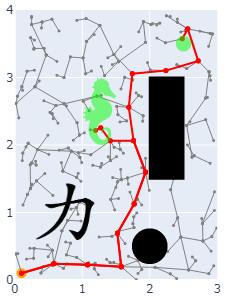
\includegraphics[width=\textwidth]{links/rectangle_basic.png}
				\caption{RRT Basic.}
			\end{minipage}
			\hfill
			\begin{minipage}[b]{0.4\textwidth}
				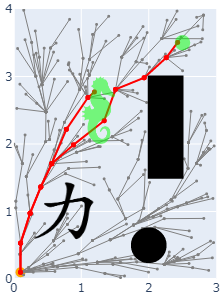
\includegraphics[width=\textwidth]{links/rectangle_star.png}
				\caption{RRT*.}
			\end{minipage}
		\end{figure}

The results text file would look like this: 
\verbatiminput{links/rectangle_mixed_goals_obstacles_basic.txt}

The Solution Path(s) are a list of the indices of the vertices that make up the solution path in order. The Solution Vertices are then printed such that the user does not need to search through the entire list of vertices to get the solution coordinates. The Solution Vertices lists the coordinates of the vertices corresponding to the solution path. Finally, the cumulative cost for the solution path is printed. If a solution is not found given the specified number of trials, then nan will be printed for all three fields. 

The table below summarizes the total costs for the solutions found using the two different algorithms.

		\begin{table}[H]
	\centering
	{\tabulinesep=2.0mm
		\begin{tabu}{ccc}
			\hline
			Solution Path & Basic RRT (Cost)     & RRT* (Cost)          \\ \hline
			1             & 26.093 & 12.571 \\ \hline
			2             & 45.169 & 24.916 \\ \hline
		\end{tabu}
	}
	\caption{\label{tab:rectangle_cost}Total cost (distance) for each solution using the Basic RRT algorithm versus the RRT* algorithm.}
\end{table}

\subsubsection{Complex Circular Domain}

This next example utilizes a circular domain with a large number of trials. There are obstacles and goals of each type. The large number of trials allows for the RRT* algorithm to find a very efficient solution, one that is almost a perfectly straight line.


		\begin{figure}[H]
	\centering
	\begin{minipage}[b]{0.4\textwidth}
		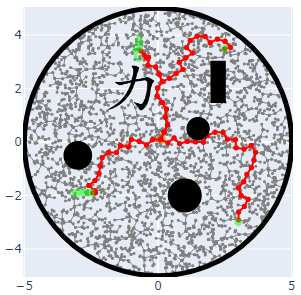
\includegraphics[width=\textwidth]{links/circle_basic.png}
		\caption{RRT Basic.}
	\end{minipage}
	\hfill
	\begin{minipage}[b]{0.4\textwidth}
		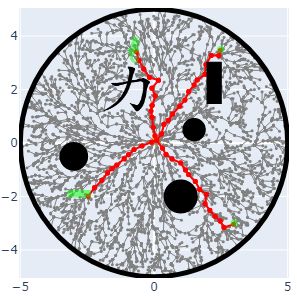
\includegraphics[width=\textwidth]{links/circle_star.png}
		\caption{RRT*.}
	\end{minipage}
\end{figure}

The results of the costs of the solutions found with the two different algorithms are shown in Table~\ref{tab:circle_cost}. The following are the key takeaways:
\begin{enumerate}
	\item There is a significant decrease in the final solution cost from using the RRT* algorithm.
	\item The step size plays a large role in finding goals that are relatively small. Some vertices will be very close to the goal, but not count as a valid solution because it is not inside the goal and a longer path is chosen.
\end{enumerate}

\begin{table}[H]
	\centering
	{\tabulinesep=2.0mm
		\begin{tabu}{ccc}
			\hline
			Solution Path & Basic RRT (Cost)     & RRT* (Cost)          \\ \hline
			1             & 38.593 & 23.626 \\ \hline
			2             & 82.726 & 35.132 \\ \hline
			3             & 40.171 & 19.396 \\ \hline
			4             & 97.500 &  38.963 \\ \hline
		\end{tabu}
	}
	\caption{\label{tab:circle_cost}Total cost (distance) for each solution using the Basic RRT algorithm versus the RRT* algorithm.}
\end{table}



\newpage
\section{Code Profiling}
A vanilla code profiling was performed to identify the bottle-neck functions or classes and improvements were incorporated where possible. An initial picture of the whole program is captured by timing various combination of domain, obstacles and path finding algorithm. To avoid coupling between various elements only one obstacle was used during the profiling process. Further, the output class was not included as it does not form the core of the software. The profiling was performed on a Ubuntu machine. In all these cases, the following parameters were kept constant:
\begin{enumerate}
\item The number of steps for which the program was run.
\item The step size for the algorithms.
\item Neighborhood size for the RRT* algorithm.
\item The origin and goal was the same.
\item The bounding box for each obstacle was the same.
\end{enumerate}
\begin{table}[H]
\centering
{\tabulinesep=2.0mm
\begin{tabu}{c c c c}
		\hline
		Algorithm & Domain & Obstacle & Total time (s) \\
		\hline
		\multirow{4}{*}{Basic RRT} & Rectangle & Rectangle  &  45.7\\
		& Rectangle & Circle  & 47.6\\
		& Rectangle & Seahorse  & 398.3\\
		& Rectangle & Force  & 62.2\\
		\hline
		\multirow{4}{*}{Basic RRT} & Circle & Rectangle  &  46.9\\
		& Circle & Circle  & 46.2\\
		& Circle & Seahorse  & 413.3\\
		& Circle & Force  & 58.8\\
		\hline
		\multirow{4}{*}{RRT*} & Circle & Rectangle  &  48.2\\ 
		& Circle & Circle  & 47.3\\
		& Circle & Seahorse  & 869.5\\
		& Circle & Force  & 77.4\\
		\hline
\end{tabu}
}
\caption{\label{tab:tot_time_original}Total time to run various combination of domain, obstacle and solution algorithm. Note: The total time is the average of 3 runs}
\end{table}
The results of the timing are shown in Table~\ref{tab:tot_time_original}. The following are the key takeaways:
\begin{enumerate}
\item There is no significant difference between the timing for circle or rectangle obstacles. This indicates that the efficiency of the analytical tests to check if a point is inside the shape or to check if the edge connecting two points intersect the shape are comparable.
\item The free form shape implementation is comparably more computationally expensive than the geometric shapes.
\end{enumerate}
\subsection{Summary of Hotspots}
The profiling of the was performed using \textit{cProfile}. The key functions identified for improvement are shown in Table~\ref{tab:functions_original}
\begin{table}[H]
\centering
{\tabulinesep=2.0mm
\begin{tabu}{c c}
		\hline
		Function & Total time spent(s) \\
		\hline
		vertex.py:61(find\_nearest\_vertex) & 21.0 \\
		shape\_free\_form.py:91(is\_point\_inside) & 158.8 \\
		\hline
\end{tabu}
}
\caption{\label{tab:functions_original} Average total time spent in bottleneck functions for 2000 basic RRT steps. For free form the average time is that of the seahorse obstacle}
\end{table}

One common in these functions were the implementation of the for loops. So wherever possible, the for loops were replaced with slicing of the numpy array. The two functions were replaced as shown below.
\begin{enumerate}
\item The original code for Vertex.find\_nearest\_vertex()
\begin{lstlisting}[language=python]
def find_nearest_vertex(self,vertex_list,new_q):
	dist_new = 0.0
	shortest_distance = float('+inf') 
	shortest_index = 0	
	for i, vertex in enumerate(vertex_list):
		if any(x == True for x in np.isnan(vertex)):
			break 
		else:
			dist_new = np.linalg.norm(new_q - vertex)
			if dist_new < shortest_distance:					
				shortest_distance = dist_new
				shortest_index = i		
	return shortest_index, shortest_distance
\end{lstlisting}
The improved code
\begin{lstlisting}[language=python]
def find_nearest_vertex(self,vertex_list,new_q):
	existing_vertex_list = vertex_list[~np.isnan(vertex_list).any(axis=1)]
	dist_norm = np.linalg.norm(existing_vertex_list-new_q, axis = 1)
	return np.argmin(dist_norm), dist_norm[np.argmin(dist_norm)]
\end{lstlisting}

\item The original code for free\_form.is\_point\_inside()
\begin{lstlisting}[language=python]
def is_point_inside(self, point):
	if(point[0] < self.x_min_val or point[0] > self.x_max_val or point[1] < 
		self.y_min_val or point[1] > self.y_max_val):
		return False
	else:
		shape_points = self.all_points_array[self.all_points_array[:,1] < 
			point[1]+2.1*self.hy]
		shape_points = shape_points[shape_points[:,1] > point[1] -2.1*self.hy]
		number_of_shape_points = shape_points.shape[0]
		eps = 1.0e-1
		test_radius = max(self.hx,self.hy)*(2.+_eps)
		for shape_point in shape_points:
			if(np.linalg.norm(point-shape_point) <= test_radius):
			return True
		return False
\end{lstlisting}

\begin{lstlisting}[language=python]
def find_nearest_vertex(self,vertex_list,new_q):
	if(point[0] < self.x_min_val or point[0] > self.x_max_val or point[1] < 
		self.y_min_val or point[1] > self.y_max_val):
		return False
	else:
		y_band = 2.1*self.hy
		shape_points = self.all_points_array[self.all_points_array[:,1] < 
			point[1]+y_band]
		shape_points = shape_points[shape_points[:,1] > point[1] -y_band]
		_eps = 1.0e-1
		relative_distance_array = np.linalg.norm(shape_points-point, axis = 1)
		test_radius = max(self.hx,self.hy)*(2.+_eps)
		if(relative_distance_array[np.argmin(relative_distance_array)] < 
			test_radius):
			return True
		return False
\end{lstlisting}
\end{enumerate}

\subsection{Summary of Improvements}	
The above changes were sufficient to reduce the total time of the run drastically as shown in Table~\ref{tab:tot_time_improved}.
\begin{table}[H]
\centering
{\tabulinesep=2.0mm
\begin{tabu}{c c c c}
		\hline
		Algorithm & Domain & Obstacle & Total time (s) \\
		\hline
		\multirow{4}{*}{Basic RRT} & Rectangle & Rectangle  & 1.3 \\
		& Rectangle & Circle  & 1.3\\
		& Rectangle & Seahorse  & 115.4\\
		& Rectangle & Force  & 3.9\\
		\hline
		\multirow{4}{*}{Basic RRT} & Circle & Rectangle  &  1.2\\
		& Circle & Circle  & 1.2\\
		& Circle & Seahorse  & 164.9\\
		& Circle & Force  & 4.6\\
		\hline
		\multirow{4}{*}{RRT*} & Circle & Rectangle  &  2.2\\ 
		& Circle & Circle  & 2.2\\
		& Circle & Seahorse  & 466.6\\
		& Circle & Force  & 8.7\\
		\hline
\end{tabu}
}
\caption{\label{tab:tot_time_improved}Total time to run various combination of domain, obstacle and solution algorithm after improvements. Note: The total time is the average of 3 runs}
\end{table}

The corresponding time for the changed functions are shown in Table~\ref{tab:functions_improved}
\begin{table}[H]
\centering
{\tabulinesep=2.0mm
\begin{tabu}{c c}
		\hline
		Function & Total time spent(s) \\
		\hline
		vertex.py:61(find\_nearest\_vertex) & 0.1 \\
		shape\_free\_form.py:91(is\_point\_inside) & 112.3 \\
		\hline
\end{tabu}
}
\caption{\label{tab:functions_improved} Average total time spent in bottleneck functions for 2000 basic RRT steps. For free form the average time is that of the seahorse obstacle}
\end{table}
The key lesson learned through this exercise is to avoid for loops when dealing with {\ttfamily numpy} arrays and use slicing instead.	

\end{document}
